\documentclass[10pt,a4paper]{article}
\usepackage[utf8]{inputenc}
\usepackage[T1]{fontenc}
\usepackage[ngerman]{babel}
\usepackage{amsmath}
\usepackage{amsfonts}
\usepackage{amssymb}
\usepackage{graphicx}


\author{Gruppe 02}
\title{Pflichtenheft}
\begin{document}

	\subsection{Statistik Funktion}
	\begin{figure}[h]
		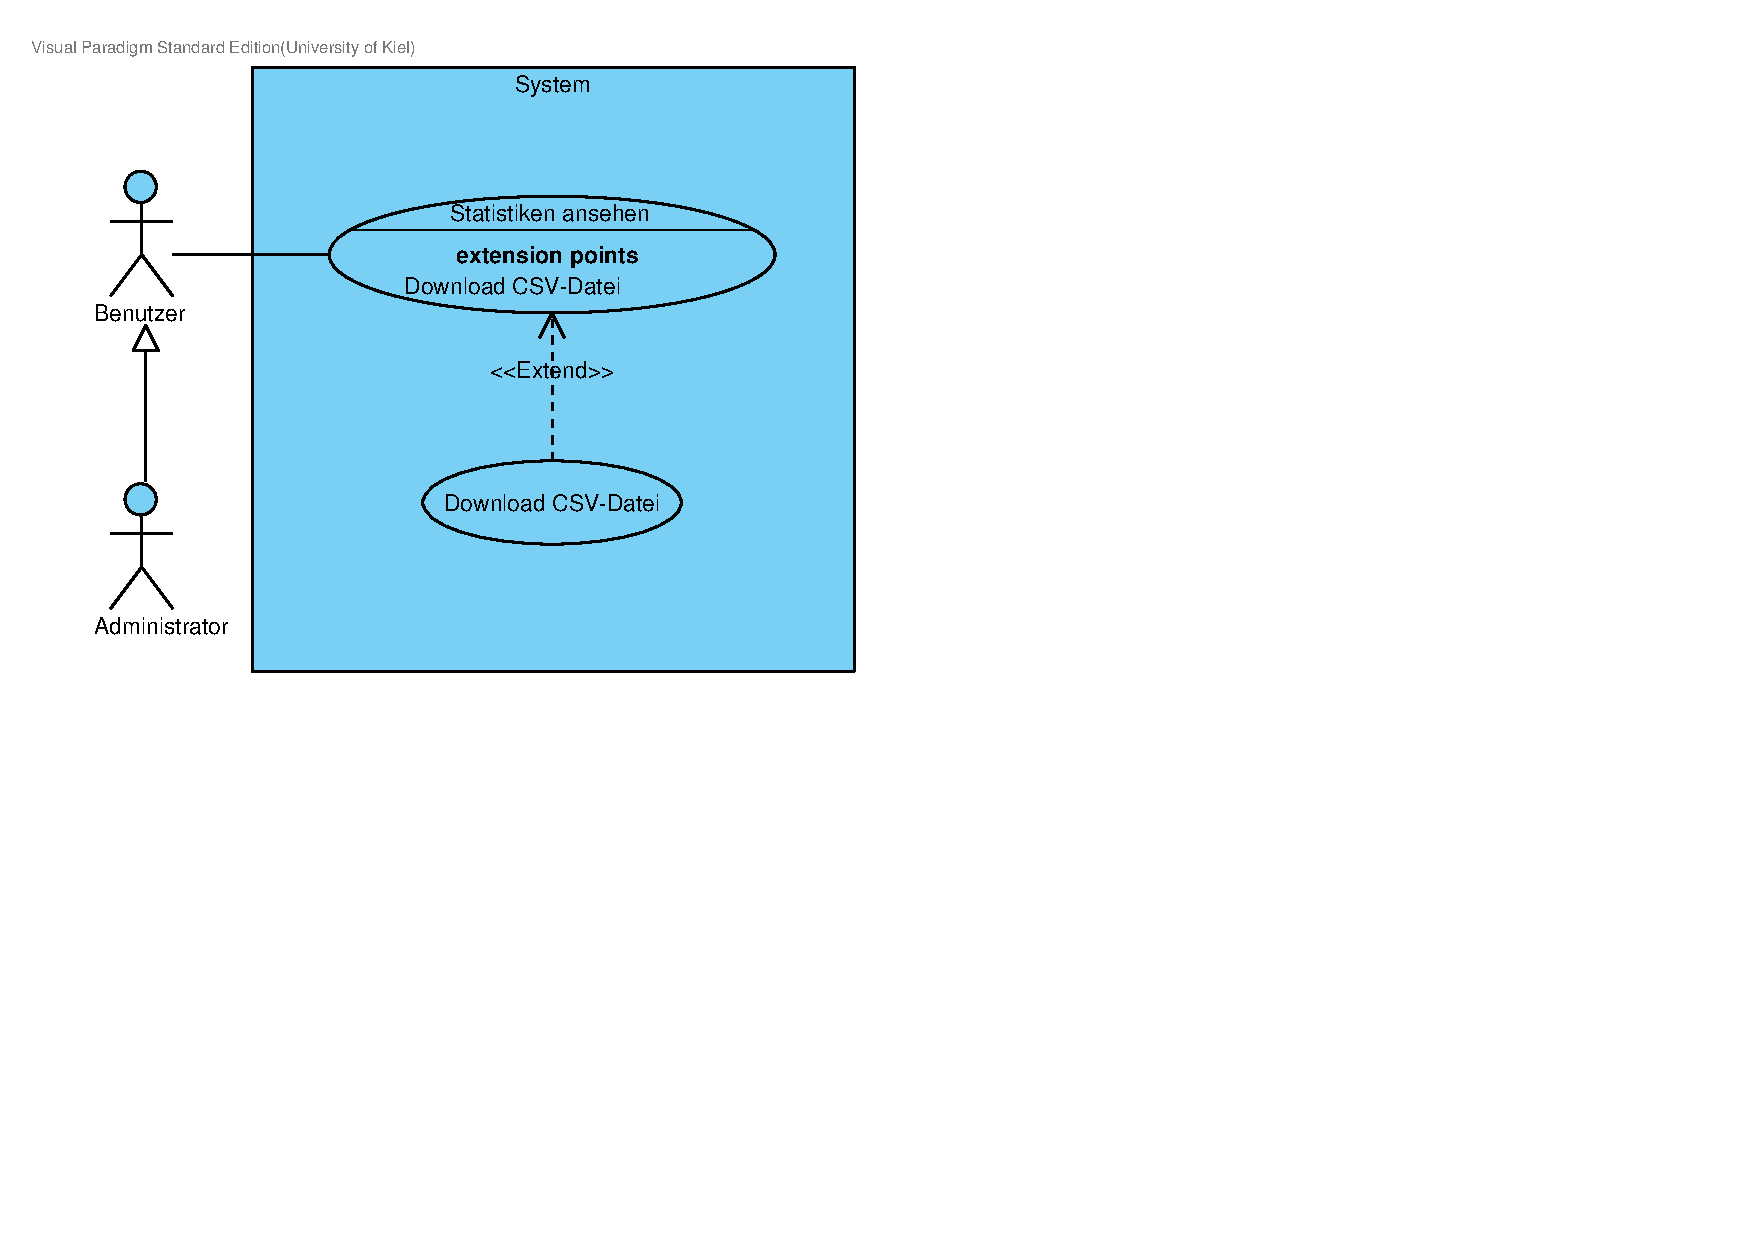
\includegraphics[width=\linewidth]{gfx/webseite/statistikfunktion.pdf}
	\end{figure}
	\subsubsection{Sehen Statistiken}
	\begin{tabular}{|l|p{.5\linewidth}|}
	\hline Use Case Nummer & - \\ 
	\hline Use Case Name & Sehen Statistiken \\ 
	\hline Initiierender Akteur & Admin and User \\
	\hline Weitere Akteure &  \\
	\hline Kurzbeschreibung & All Users can see a graphical representation of selected anonymous statistics. \\
	\hline Vorbedingung & eingeloggt \\
	\hline Nachbedingung &   \\
	\hline \multicolumn{2}{|c|}{Funktionalität des UseCases}\\
	\hline Ablauf & \begin{itemize}
			\item User or Admin select the statistic they would like to view:
				\begin{enumerate}
					\item Number of visitors
					\item Points aquired
					\item Number of activites completed
					\item Most popular activities
				\end{enumerate}
			\item User or Admin give a timeframe to generate the statistics within.
		\end{itemize} \\
	\hline Alternativen &  \\
	\hline Ausnahmen & An error is given if either the two dates entered to use as a timeframe are invalid. \\
	\hline Benutzte Use Cases & \begin{itemize} 
		\item Eingeben Zeitraum
		\item Ansicht Grafik Auf
Besucheranzahl
\item Ansicht Grafik Auf
Gesammelte Punkte
\item Ansicht Grafik Auf Erledigte Aktivitaten
\item Ansicht Grafik Auf Beliebteste Activitaten
	\end{itemize} \\
	\hline \multicolumn{2}{|c|}{Weitere Informationen} \\
	\hline Spezielle Anforderungen &  \\
	\hline Annahmen & It has been assumed that the time frame given to generate the graph from has been given as two dates as opposed to two datetime format inputs. \\
	\hline
	\end{tabular}
	
	\subsubsection{Download CSV-Datei}
	\begin{tabular}{|l|p{.5\linewidth}|}
	\hline Use Case Nummer & - \\ 
	\hline Use Case Name & Download CSV-Datei \\ 
	\hline Initiierender Akteur & Admin and User \\
	\hline Weitere Akteure &  \\
	\hline Kurzbeschreibung & All Users can download a .csv copy of the anonymous statistics. \\
	\hline Vorbedingung & eingeloggt \\
	\hline Nachbedingung &   \\
	\hline \multicolumn{2}{|c|}{Funktionalität des UseCases}\\
	\hline Ablauf & User or Admin click the download link on statistics page of the website. \\
	\hline Alternativen &  \\
	\hline Ausnahmen &  \\
	\hline Benutzte Use Cases &  \\
	\hline \multicolumn{2}{|c|}{Weitere Informationen} \\
	\hline Spezielle Anforderungen &  \\
	\hline Annahmen & It has been assumed that the .csv file is not dynamically generated and is just an output of all statistics. \\
	\hline
	\end{tabular}
	
\end{document}